\documentclass[border=3pt]{standalone}
\usepackage{times}
\usepackage{amsmath,bm}
\usepackage{tikz}
\usetikzlibrary{positioning,arrows.meta,fit,calc}
\begin{document}
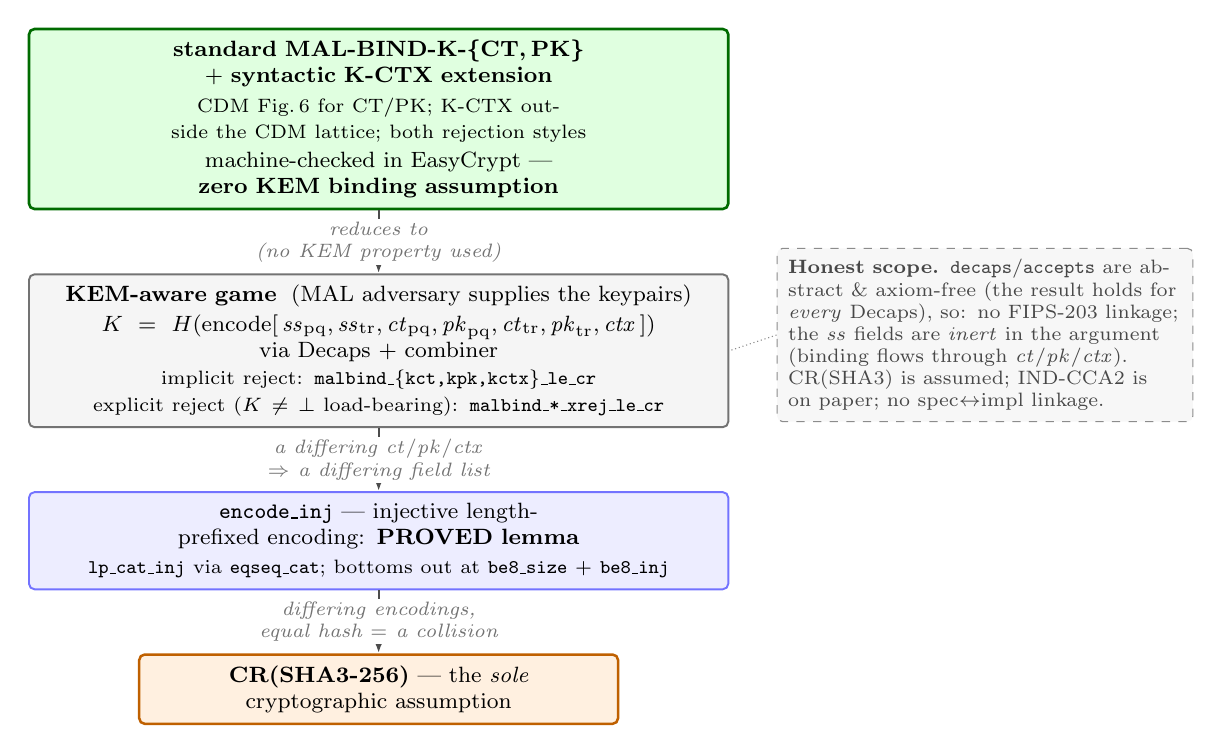
\begin{tikzpicture}[
  font=\footnotesize, >={Latex[length=4pt]},
  box/.style={draw, rounded corners=2pt, align=center, inner sep=4pt, line width=0.7pt, text width=86mm},
  result/.style={box, fill=green!12, draw=green!42!black, line width=0.95pt},
  mid/.style={box, fill=black!4, draw=black!55},
  lemma/.style={box, fill=blue!7, draw=blue!55},
  assume/.style={box, fill=orange!12, draw=orange!75!black, line width=0.9pt, text width=58mm},
  redu/.style={font=\scriptsize\itshape, text=black!55, align=center},
  scope/.style={draw, dashed, rounded corners=2pt, fill=black!3, draw=black!45, align=left,
                inner sep=4pt, font=\scriptsize, text=black!72, text width=50mm},
]
% ---- result (top) ----
\node[result] (res)
  {\textbf{standard MAL-BIND-K-\{CT,\,PK\} $+$ syntactic K-CTX extension}\\[1pt]
   {\scriptsize CDM Fig.\,6 for CT/PK; K-CTX outside the CDM lattice; both rejection styles}\\[1pt]
   machine-checked in EasyCrypt --- \textbf{zero KEM binding assumption}};
% ---- KEM-aware game ----
\node[mid, below=8mm of res] (game)
  {\textbf{KEM-aware game} \;(MAL adversary supplies the keypairs)\\[1pt]
   $K = H(\mathrm{encode}[\,\mathit{ss}_{\mathrm{pq}}, \mathit{ss}_{\mathrm{tr}},
   \mathit{ct}_{\mathrm{pq}}, \mathit{pk}_{\mathrm{pq}}, \mathit{ct}_{\mathrm{tr}},
   \mathit{pk}_{\mathrm{tr}}, \mathit{ctx}\,])$ \;via Decaps + combiner\\[2pt]
   {\scriptsize implicit reject: \texttt{malbind\_\{kct,kpk,kctx\}\_le\_cr}\\
   explicit reject ($K\!\neq\!\bot$ load-bearing): \texttt{malbind\_*\_xrej\_le\_cr}}};
% ---- encode_inj ----
\node[lemma, below=8mm of game] (enc)
  {\textbf{\texttt{encode\_inj}} --- injective length-prefixed encoding: \textbf{PROVED lemma}\\[1pt]
   {\scriptsize \texttt{lp\_cat\_inj} via \texttt{eqseq\_cat}; bottoms out at \texttt{be8\_size} + \texttt{be8\_inj}}};
% ---- assumption (bottom) ----
\node[assume, below=8mm of enc] (cr)
  {\textbf{CR(SHA3-256)} --- the \emph{sole} cryptographic assumption};
% ---- reduction arrows (downward) ----
\draw[->, line width=0.8pt, black!70] (res) -- (game)
  node[midway, redu, fill=white, inner sep=1pt] {reduces to\\(no KEM property used)};
\draw[->, line width=0.8pt, black!70] (game) -- (enc)
  node[midway, redu, fill=white, inner sep=1pt] {a differing $\mathit{ct}/\mathit{pk}/\mathit{ctx}$\\$\Rightarrow$ a differing field list};
\draw[->, line width=0.8pt, black!70] (enc) -- (cr)
  node[midway, redu, fill=white, inner sep=1pt] {differing encodings,\\equal hash $=$ a collision};
% ---- honest scope (side) ----
\node[scope, right=6mm of game.east, anchor=west, yshift=2mm] (scope)
  {\textbf{Honest scope.} \texttt{decaps}/\texttt{accepts} are abstract \& axiom-free
   (the result holds for \emph{every} Decaps), so: no FIPS-203 linkage; the
   $\mathit{ss}$ fields are \emph{inert} in the argument (binding flows through
   $\mathit{ct}/\mathit{pk}/\mathit{ctx}$). CR(SHA3) is assumed; IND-CCA2 is on paper;
   no spec$\leftrightarrow$impl linkage.};
\draw[densely dotted, black!45] (scope.west) -- (game.east);
\end{tikzpicture}
\end{document}
